\documentclass[11pt,a4paper]{article}
\usepackage[margin=2.2cm]{geometry}
\usepackage{fontspec}
\usepackage{booktabs}
\usepackage{array}
\usepackage{tabularx}
\usepackage{longtable}
\usepackage{hyperref}
\usepackage{xcolor}
\usepackage{enumitem}
\usepackage{titlesep}
\usepackage{titlesec}
\usepackage{fancyhdr}
\usepackage{graphicx}
\usepackage{amssymb}

\setmainfont{Times New Roman}
\definecolor{headingblack}{HTML}{000000}
\definecolor{lightgray}{HTML}{F2F4F7}
\hypersetup{colorlinks=true, linkcolor=headingblack, urlcolor=headingblack, citecolor=headingblack}
\titleformat{\section}{\Large\bfseries\color{headingblack}}{\thesection}{0.8em}{}
\titleformat{\subsection}{\large\bfseries\color{headingblack}}{\thesubsection}{0.8em}{}
\setlist[itemize]{leftmargin=1.4em}
\setlist[enumerate]{leftmargin=1.6em}
\pagestyle{fancy}
\setlength{\headheight}{14pt}
\fancyhf{}
\lhead{iBEC International Bioinformatics Engineering Competition}
\rhead{Project Report}
\cfoot{\thepage}

\graphicspath{{figures/}}

\begin{document}

\begin{center}
{\LARGE\bfseries CygnusX: A Multi-Agent Platform for Reproducible Computational Experiments in Omics Analysis}\\[1.0em]
\end{center}

\begin{tabularx}{\textwidth}{>{\bfseries}p{0.24\textwidth}X}
\toprule
Team ID & \texttt{IBEC26-35}\\
Project Title & CygnusX: A Multi-Agent Platform for Reproducible Computational Experiments in Omics Analysis\\
Team Name & \texttt{CygnusX}\\
Institution & Huazhong Agricultural University\\
Team Members & \texttt{[add members and roles]}\\
Track / Category & Bioinformatics / AI for Science Research Platform\\
Date & 2026-09-22\\
\bottomrule
\end{tabularx}

\section*{Executive Summary}

Omics big data is a core driver for decoding complex living systems and for bridging genotype to phenotype (G-to-P). Yet life-science research currently faces a deep-seated \textbf{reproducibility crisis in computational experiments combined with a cognitive-overload bottleneck}: researchers are trapped in the tedious configuration of heterogeneous toolchains and the long-chain tuning of parameters, analysis remains a black box, and the evidence chain is fragmented; and when general-purpose large models are used to generate analysis code end to end, the result falls into the fatal defects of ``statistical hallucination, non-auditability, and lack of biological-logic constraints''.

To address these challenges we present \textbf{CygnusX}, a multi-agent research platform for reproducible computational experiments in omics analysis. The platform proposes a \textbf{``Decoupled Reasoning \& Deterministic Execution''} methodology:

\begin{enumerate}
  \item \textbf{Scientific multi-agent collaboration network}: 18 domain-specialized agents (covering hypothesis deconstruction, multi-omics pipeline orchestration, quality auditing, and causal inference) cooperatively drive 38 atomic scientific Skills with strict input/output contracts and semantic constraints;
  \item \textbf{Deterministic trusted scientific computing base}: the fragile path of ``letting the model generate scripts without constraint'' is rejected outright; every computation is strictly anchored in containerized workflow assets formally validated by domain experts;
  \item \textbf{Provenance Capsule for the full life cycle of a computational experiment}: each analysis automatically captures the global parameter topology, runtime image hash, algorithm random seed, intermediate-state fingerprints (MD5), and a re-runnable execution graph, enabling machine self-verification of research evidence.
\end{enumerate}

In a real agricultural-biology case (mining multi-omics targets in the plant pathogen response), CygnusX realizes a complete closed loop from natural-language scientific hypothesis, through dynamic planning of cross-omics computational experiments and rigorous whole-chain quality self-correction, to core candidate regulatory genes and causal evidence-chain aggregation. The system substantially lowers the engineering cognitive load on life-science researchers and shortens the reconstruction cycle of conventional long-chain computational experiments by more than 80\%, providing a high-rigor, strongly interpretable infrastructure paradigm for AI-empowered basic life science and breeding research.

\textbf{Keywords:} AI for Science; bioinformatics; multi-agent systems; computational experiments; reproducibility; evidence-chain graph; omics mining

\section{Research Background and Scientific Pain Points}

Modern life science, modern breeding, and precision medicine have fully entered the new paradigm of ``data-driven scientific discovery''. From transcriptomics (RNA-seq) and epigenomics (ATAC-seq/ChIP-seq) to single-cell and spatiotemporal omics, massive multi-omics data provide an unprecedented panorama for resolving gene regulatory networks and mining key trait targets. However, transforming massive raw sequencing data into statistically rigorous and biologically insightful conclusions still confronts a severe ``cognitive and methodological gap'' in real research practice:

\begin{verbatim}
scientific question and experimental phenotype
  | (pain point 1: high cognitive load)
multi-omics computational experiment design and heterogeneous toolchain orchestration
  | (pain point 2: batch effects and blind spots in quality control)
high-throughput pipeline processing and multi-dimensional quality governance
  | (pain point 3: narrow hypothesis space and slow incremental iteration)
cross-omics evidence aggregation and causal inference on candidate targets
  | (pain point 4: reproducibility crisis and broken evidence chain)
rigorous publication / wet-lab cross-validation
\end{verbatim}

\subsection{Engineering cognitive load of complex multi-omics computational experiments blocks scientific innovation}

Standard omics analysis spans sample QC, read alignment, transcript quantification, differential statistical modeling, functional enrichment, and network deconvolution. In conventional practice, researchers navigate hundreds of parameter combinations, environment dependencies, and complex command-line scripts, with a single pipeline configuration taking hours on average. Configuration omissions and metadata format errors surface only after substantial compute has been consumed, spending researchers' precious effort on ``fixing environments and tuning parameters'' and severely squeezing the space for exploring frontier hypotheses.

\subsection{Statistical false positives decoupled from quality governance}

High-throughput sequencing is strongly affected by library-construction bias, nucleic-acid degradation, and batch effects. Conventional pipelines rely on human experience for post-hoc inspection after analysis and lack active quality governance during computation; once a low-quality library infiltrates differential analysis or cross-omics integration, it readily generates large numbers of statistical false positives, misleading subsequent costly wet-lab validation.

\subsection{Slow hypothesis-space exploration and blocked incremental iteration}

When researchers need to explore fine-grained biological subtypes, switch comparison models, adjust non-specific filtering thresholds, or introduce epigenetic constraints, conventional analysis often requires rewriting the entire pipeline. This high-friction interaction cost leads researchers toward conservative preset flows and makes it difficult to carry out sufficient parameter-sensitivity probing and incremental mining for complex hypotheses.

\subsection{The ``reproducibility crisis'' of computational experiments}

\emph{Nature} has repeatedly warned about the computational reproducibility predicament in life science: at publication time the dynamic software sources on which the original scripts depended can no longer be resolved, reference-genome annotation versions are ambiguous, random seeds are lost, and intermediate files are unverified. After staff turnover, laboratories even have to conduct ``research archaeology'' from historical chat logs and incomplete code, severely weakening the credibility of published findings.

\subsection{General generative AI is a poor fit for rigorous science}

Large language models show strong potential in natural-language understanding and code generation, but letting them generate bioinformatics analysis code end to end readily produces the fatal problem of ``code that looks reasonable yet introduces hidden biological errors'' (for example, confusing non-normal distribution models, omitting sequencing-depth normalization, or misreading the degrees of freedom of a statistical test). In rigorous research and publication settings, code that has not passed peer review must never serve as the basis for scientific computation.

\section{System Design Philosophy and Research Positioning}

\subsection{Core design philosophy: Decoupled Reasoning \& Deterministic Execution}

To resolve the fundamental contradiction between the ``generative freedom'' of large models and the ``deterministic reproducibility'' required by scientific research, CygnusX establishes the architectural principle of \textbf{``AI is responsible for scientific reasoning and orchestration; expert assets are responsible for deterministic physical computation''}:

\begin{verbatim}
+-------------------------------------------------------------------------+
|   upper layer: scientific cognition and reasoning network (AI freedom)   |
|  hypothesis understanding -> experiment planning -> role review         |
|  -> result interpretation and hypothesis iteration                       |
+-------------------------------------------------------------------------+
   strict API semantic contracts and quality gates
+-------------------------------------------------------------------------+
|  lower layer: deterministic scientific computing base (expert assets)    |
|  expert-validated workflow (Snakemake) -> container image snapshot       |
|  -> statistically rigorous algorithms -> provenance capsule             |
+-------------------------------------------------------------------------+
\end{verbatim}

\begin{itemize}
  \item \textbf{Upper cognitive system}: a multi-agent collaboration network built on large models endowed with life-science domain knowledge, responsible for hypothesis deconstruction, semantic task routing, parameter reasoning proposals, multi-dimensional quality review, and integrated biological interpretation of evidence.
  \item \textbf{Lower computing kernel}: the unconstrained shell write permission and ad-hoc code-construction permission of agents are firmly blocked. Every computational task must map to a standardized workflow and atomic scientific Skill that has undergone strict peer review and statistically rigorous methodology.
  \item \textbf{Boundary criterion}: computation is never improvised by the model, and the model never oversteps to replace human scientists in drawing conclusions; what an agent outputs is a ``causal evidence recommendation with confidence and boundary conditions'', while final decision authority and wet-lab design belong to researchers.
\end{itemize}

\subsection{Research positioning and capability evolution}

\begin{table}[htbp]
\centering
\renewcommand{\arraystretch}{1.25}
\begin{tabularx}{\textwidth}{p{0.10\textwidth}p{0.22\textwidth}X p{0.20\textwidth}}
\toprule
\textbf{Phase} & \textbf{Platform form} & \textbf{Key scientific and engineering capability} & \textbf{Status}\\
\midrule
Phase 1 & Deterministic workflow base & Declarative specification, versioned pipelines, containerized runtime, static preflight, deterministic QC & Base highly mature\\
Phase 2 & AI-assisted computing experiments & Scientific intent parsing, parameter topology derivation, automated Skill scheduling, anomaly diagnosis, report summarization & Current core function\\
Phase 3 & Controlled multi-agent reasoning system & Scientific contract constraints, cross-omics dynamic planning, multi-role quality audit gates, causal evidence graph & Current main achievement\\
Phase 4 & Hypothesis-driven closed-loop computational exploration & Autonomous deconstruction of scientific questions, counterfactual computational experiment design, multi-modal literature evidence cross-validation & Frontier research direction\\
\bottomrule
\end{tabularx}
\caption{Research positioning and capability evolution.}
\end{table}

\section{Overall Technical Route and System Architecture}

CygnusX follows the design principle of ``top-down scientific decomposition, bottom-up computational verification'', with the whole process built inside a transparent and auditable scientific closed loop:

\begin{verbatim}
[research question / frontier phenotype hypothesis]
  | (natural-language interaction / structured experiment design)
[intent deconstruction and preflight engine] -- check sample balance,
  |                                        batch distribution, depth, replicates
  v
[multi-agent orchestration network] -------- chief scientist agent leads,
  |                                        organizes the multi-omics experiment topology
  v
[controlled computational experiment scheduling] -- activate atomic Skills,
  |        mount containerized deterministic algorithms (DESeq2, MACS3, ...)
  v
[dynamic quality audit gate] -------- quality-audit agent applies statistical
  |        rule gates (Q30, mapping rate, FRiP)
  v
[causal evidence-chain aggregation and interpretation] -- data curator and
  |        evidence reporter produce structured candidate targets and networks
  v
[full-lifecycle provenance capsule] -------- lock code, parameters, container
           image hash, MD5, and the re-runnable graph
\end{verbatim}

\begin{verbatim}
+---------------------------------------------------------------------------------------+
|                          scientific interaction and task intake layer                  |
|   natural-language hypothesis query | experiment design sheet | project workbench      |
+---------------------------------------------------------------------------------------+
  |
+---------------------------------------------------------------------------------------+
|                          multi-agent cognition and governance system                  |
|  [general] intent-parsing agent | experiment-planning agent | science-report agent    |
|  [analysis] transcriptome agent | epigenome agent | single-cell agent                |
|             | variant-mining agent | multi-omics integration agent                    |
|  [governance] data-integrity curator | quality auditor (Quality Gate)               |
|             | evidence reporter                                                        |
+---------------------------------------------------------------------------------------+
  | (declarative JSON contracts / idempotent invocation)
+---------------------------------------------------------------------------------------+
|                       domain atomic scientific Skill library (38 Skills)               |
|  expression quantification | differential significance modeling                       |
|  | genome synteny dot plot | chromatin-open-region peak calling | GO/KEGG enrichment  |
+---------------------------------------------------------------------------------------+
  | (containerized isolated runtime)
+---------------------------------------------------------------------------------------+
|                        trusted scientific computing and data engine                    |
|   workflow engine (Snakemake/Nextflow) | containers (Docker/Singularity)            |
|   | local research storage base                                                       |
+---------------------------------------------------------------------------------------+
  |
+---------------------------------------------------------------------------------------+
|                          provenance capsule (Provenance Capsule)                       |
|  environment lockfile | artifact MD5 fingerprint | global random seed                 |
|  | topological re-run script (ReproScript)                                           |
+---------------------------------------------------------------------------------------+
\end{verbatim}

\section{Core Methodology and Key Technical Contributions}

\subsection{The ``scientific contract-driven mechanism'' of cognitive--computational decoupling}

The platform abandons the dangerous pattern of letting agents invoke the operating-system shell at will and instead imposes semantic constraints on every operation through a \textbf{``Scientific Capability Contract''}. Each Skill carries a strict mathematical and biological contract definition:

\begin{itemize}
  \item \textbf{Pre-flight invariants}: e.g., the input count matrix must contain unnormalized integer Counts; data already normalized to FPKM/TPM is strictly forbidden as input to a statistical differential-testing model;
  \item \textbf{Statistical assumptions}: e.g., biological replication $N \ge 3$ is required; if $N < 3$ the run is automatically downgraded to exploratory mode with a mandatory insufficient-statistical-power warning;
  \item \textbf{Evidence output specifications}: standardized output of effect size ($\log_2 \text{FoldChange}$), corrected significance ($P\text{-adj}$ / q-value), and model diagnostic residual plots.
\end{itemize}

\subsection{The 18-agent multi-agent research collaboration network}

The platform builds a multi-agent research community with clear roles and mutual checks, divided into a general domain, an analysis domain, and a governance domain:

\begin{enumerate}
  \item \textbf{Scientific planning and analysis domain}
  \begin{itemize}
    \item \textbf{Transcriptome agent}: expert in subtle differential enrichment, isoform expression, and unbiased co-expression network construction;
    \item \textbf{Epigenome agent}: specialized in cis-regulatory elements, chromatin accessibility (ATAC-seq), and transcription-factor binding footprint analysis;
    \item \textbf{Multi-omics integration agent}: applies matrix factorization and causal graphical models to co-localize evidence across the expression, epigenetic, and variant dimensions.
  \end{itemize}
  \item \textbf{Scientific governance domain}
  \begin{itemize}
    \item \textbf{Quality auditor}: holds a ``veto right over the experiment'', is independent of the execution logic, and gates quality using rigorous statistical indicators (sequencing contamination, principal-component dispersion, library signal-to-noise ratio);
    \item \textbf{Data curator}: responsible for reference-genome version traceability, FASTA/GTF annotation completeness checks, and sample-metadata normalization;
    \item \textbf{Evidence reporter}: assembles multi-source heterogeneous evidence into a publication-grade research report with figures and methodological descriptions.
  \end{itemize}
\end{enumerate}

\begin{figure}[htbp]
\centering
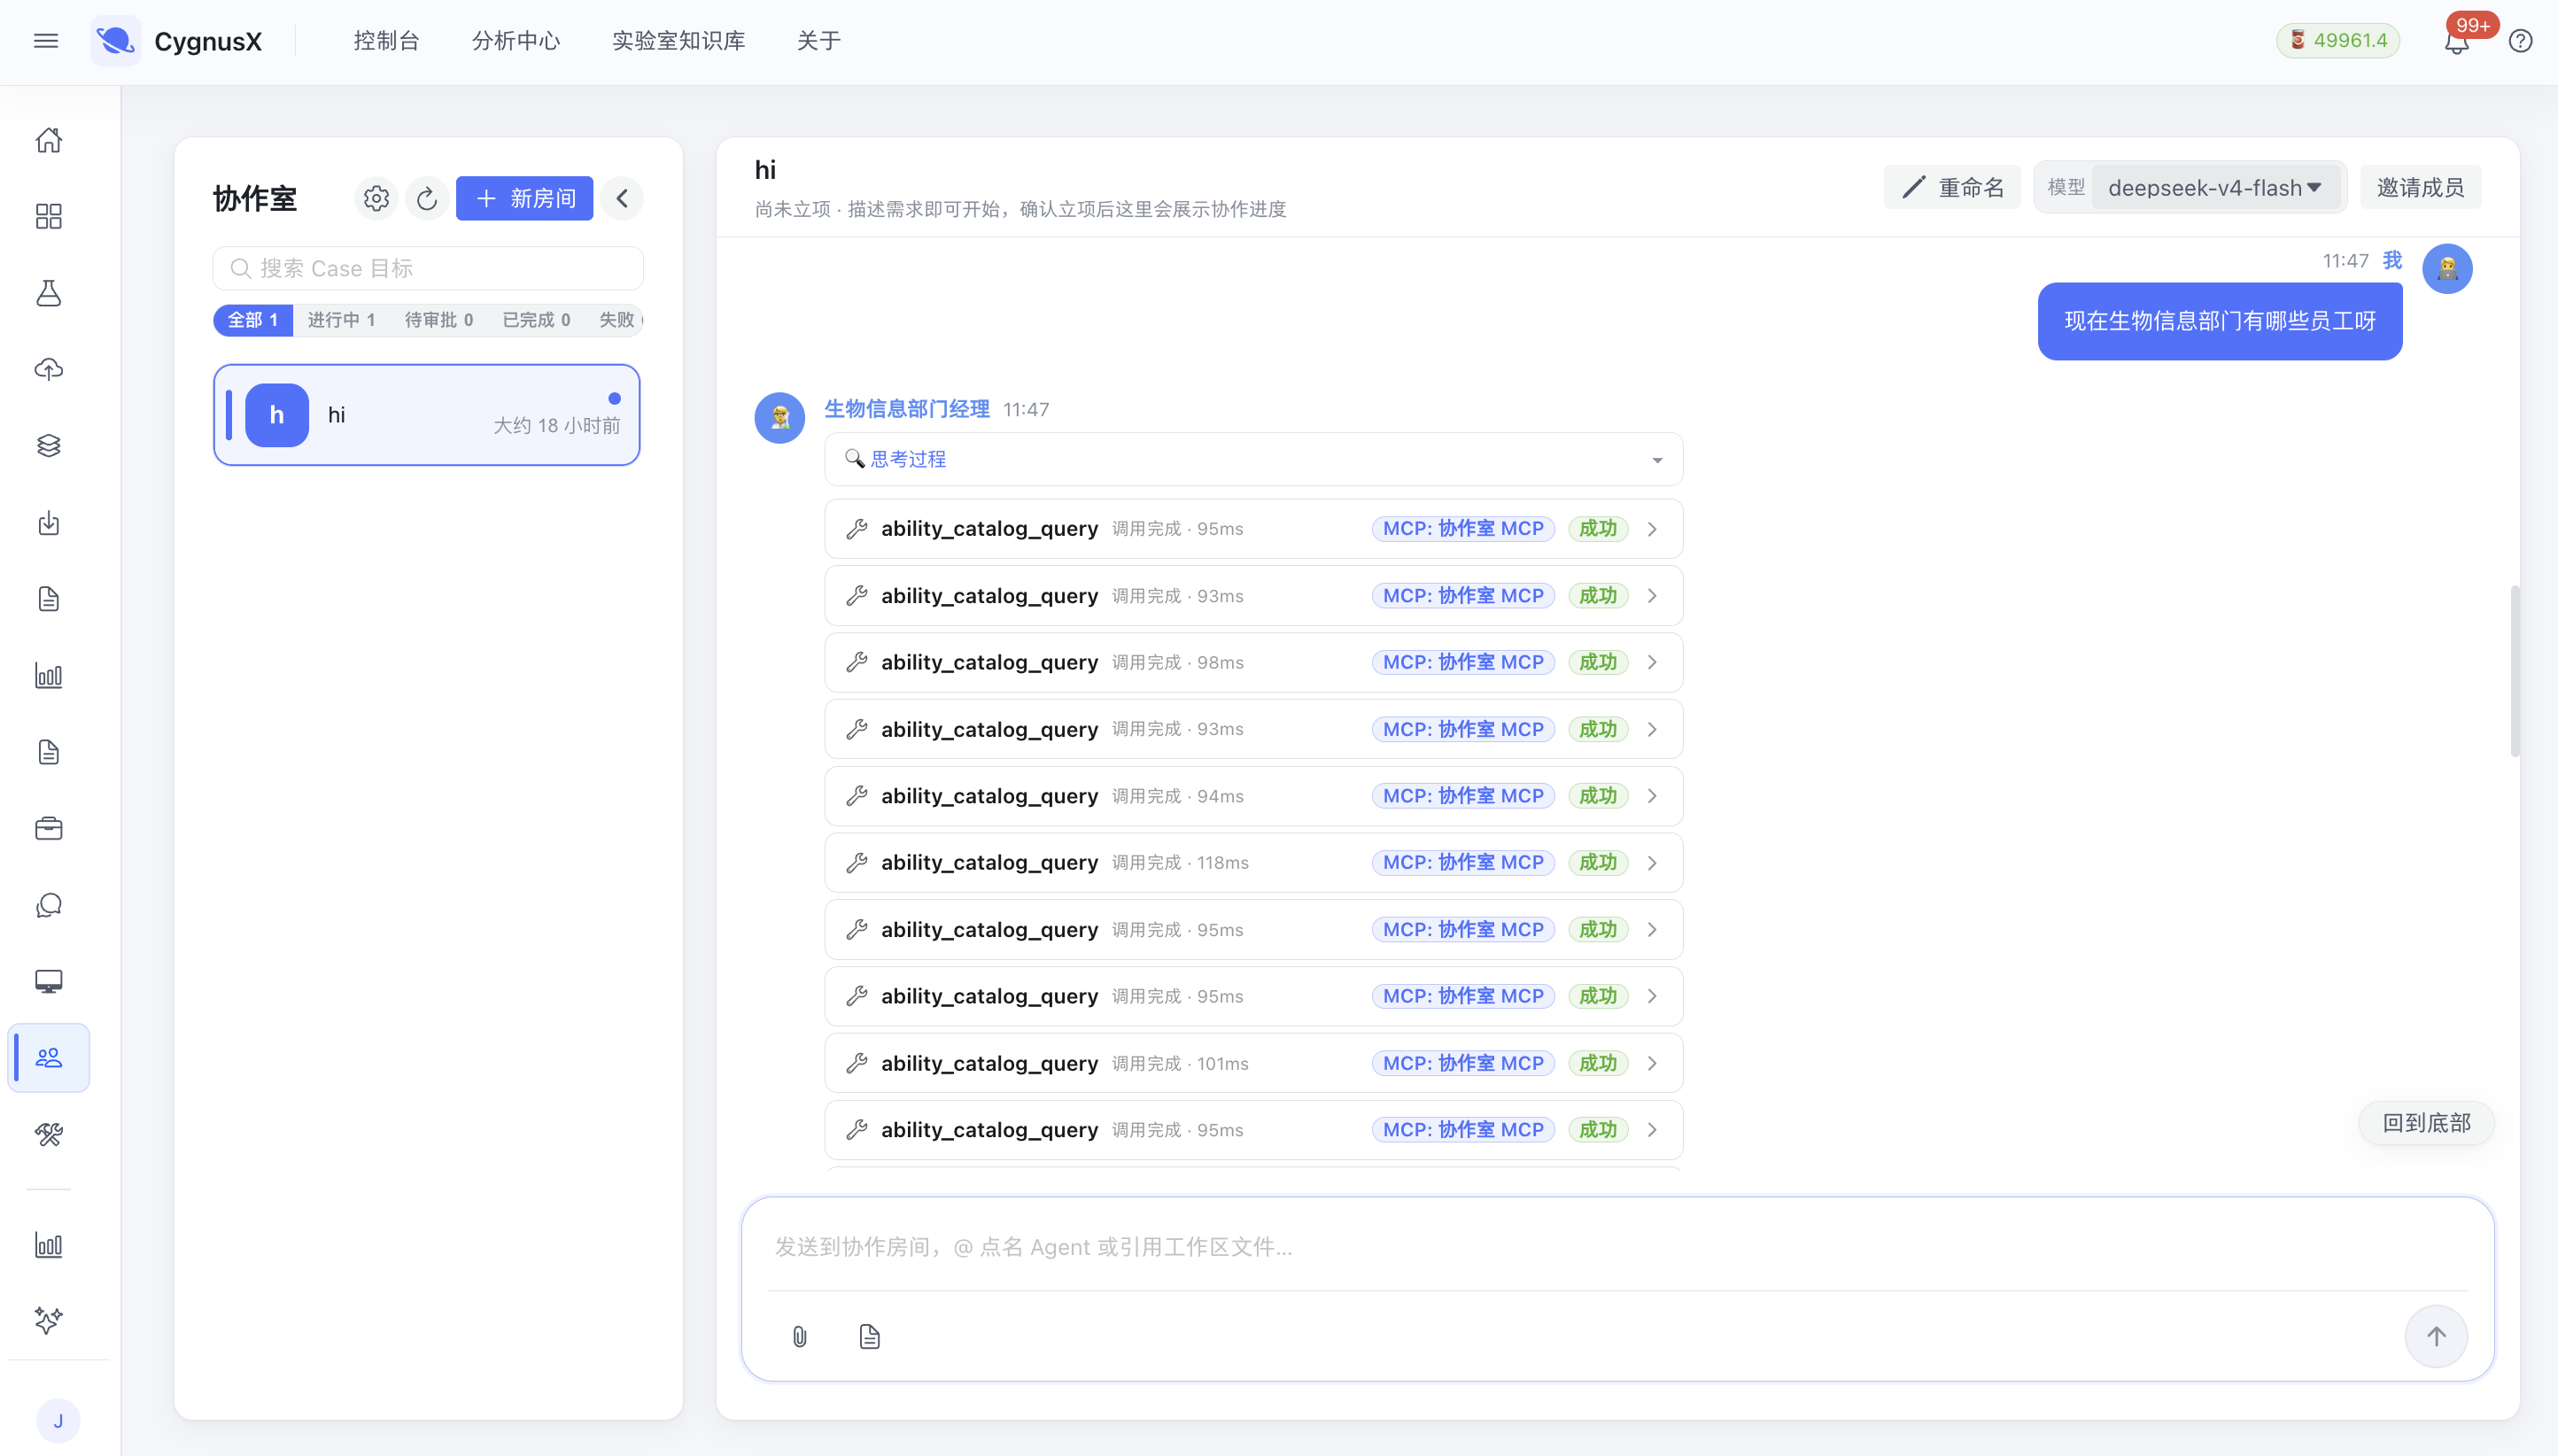
\includegraphics[width=0.95\textwidth]{fig1_multiagent_room.png}
\caption{Multi-agent collaboration in the CygnusX collaboration room. The governance-domain agent (Bioinformatics Department Manager) receives a natural-language requirement and performs capability-catalog retrieval and task dispatch through MCP tools; each tool call's name, latency, and result are recorded as structured events, supporting full auditability.}
\end{figure}

\subsection{Dynamic quality gates and experimental self-correction}

During computation, the system carries out \textbf{active quality intervention} through structured rules and agent collaboration rather than passively accepting failed results.

\textbf{Example: the library-contamination and batch-effect blocking chain.} When the FastQ Screen Skill detects nucleic-acid contamination above threshold, or when PCA analysis reveals that the first principal component is dominated by extraction batch rather than biological treatment, the \textbf{quality-audit agent immediately breaks the current pipeline}, refusing to proceed directly to downstream enrichment analysis, automatically presents a confounding-factor diagnostic plot to the researcher, and proactively recommends SVA (Surrogate Variable Analysis) or ComBat-seq correction.

\subsection{The full-lifecycle Provenance Capsule}

To fundamentally solve the ``incurable disease of irreproducibility'' in bioinformatics, CygnusX replaces the conventional practice of delivering only ``figures and Excel tables'' with an atomically sedimented \textbf{Provenance Capsule} for every task:

\begin{itemize}
  \item \textbf{Deterministic environment lock}: automatically exports the exact Conda/Singularity/Docker image SHA256 digests and dependency manifests of all invoked tools;
  \item \textbf{Data lineage graph}: adopts the W3C PROV scientific data standard to record, precisely, the mathematical transformation history from every raw FASTQ to every pixel of the final heatmap;
  \item \textbf{Independent re-run credential}: a hash-verified self-contained execution script \texttt{reproduce\_experiment.sh} accompanies the analysis package, so that any third-party laboratory can verify the numerical consistency of the conclusions with one command in a fully offline environment.
\end{itemize}

\begin{figure}[htbp]
\centering
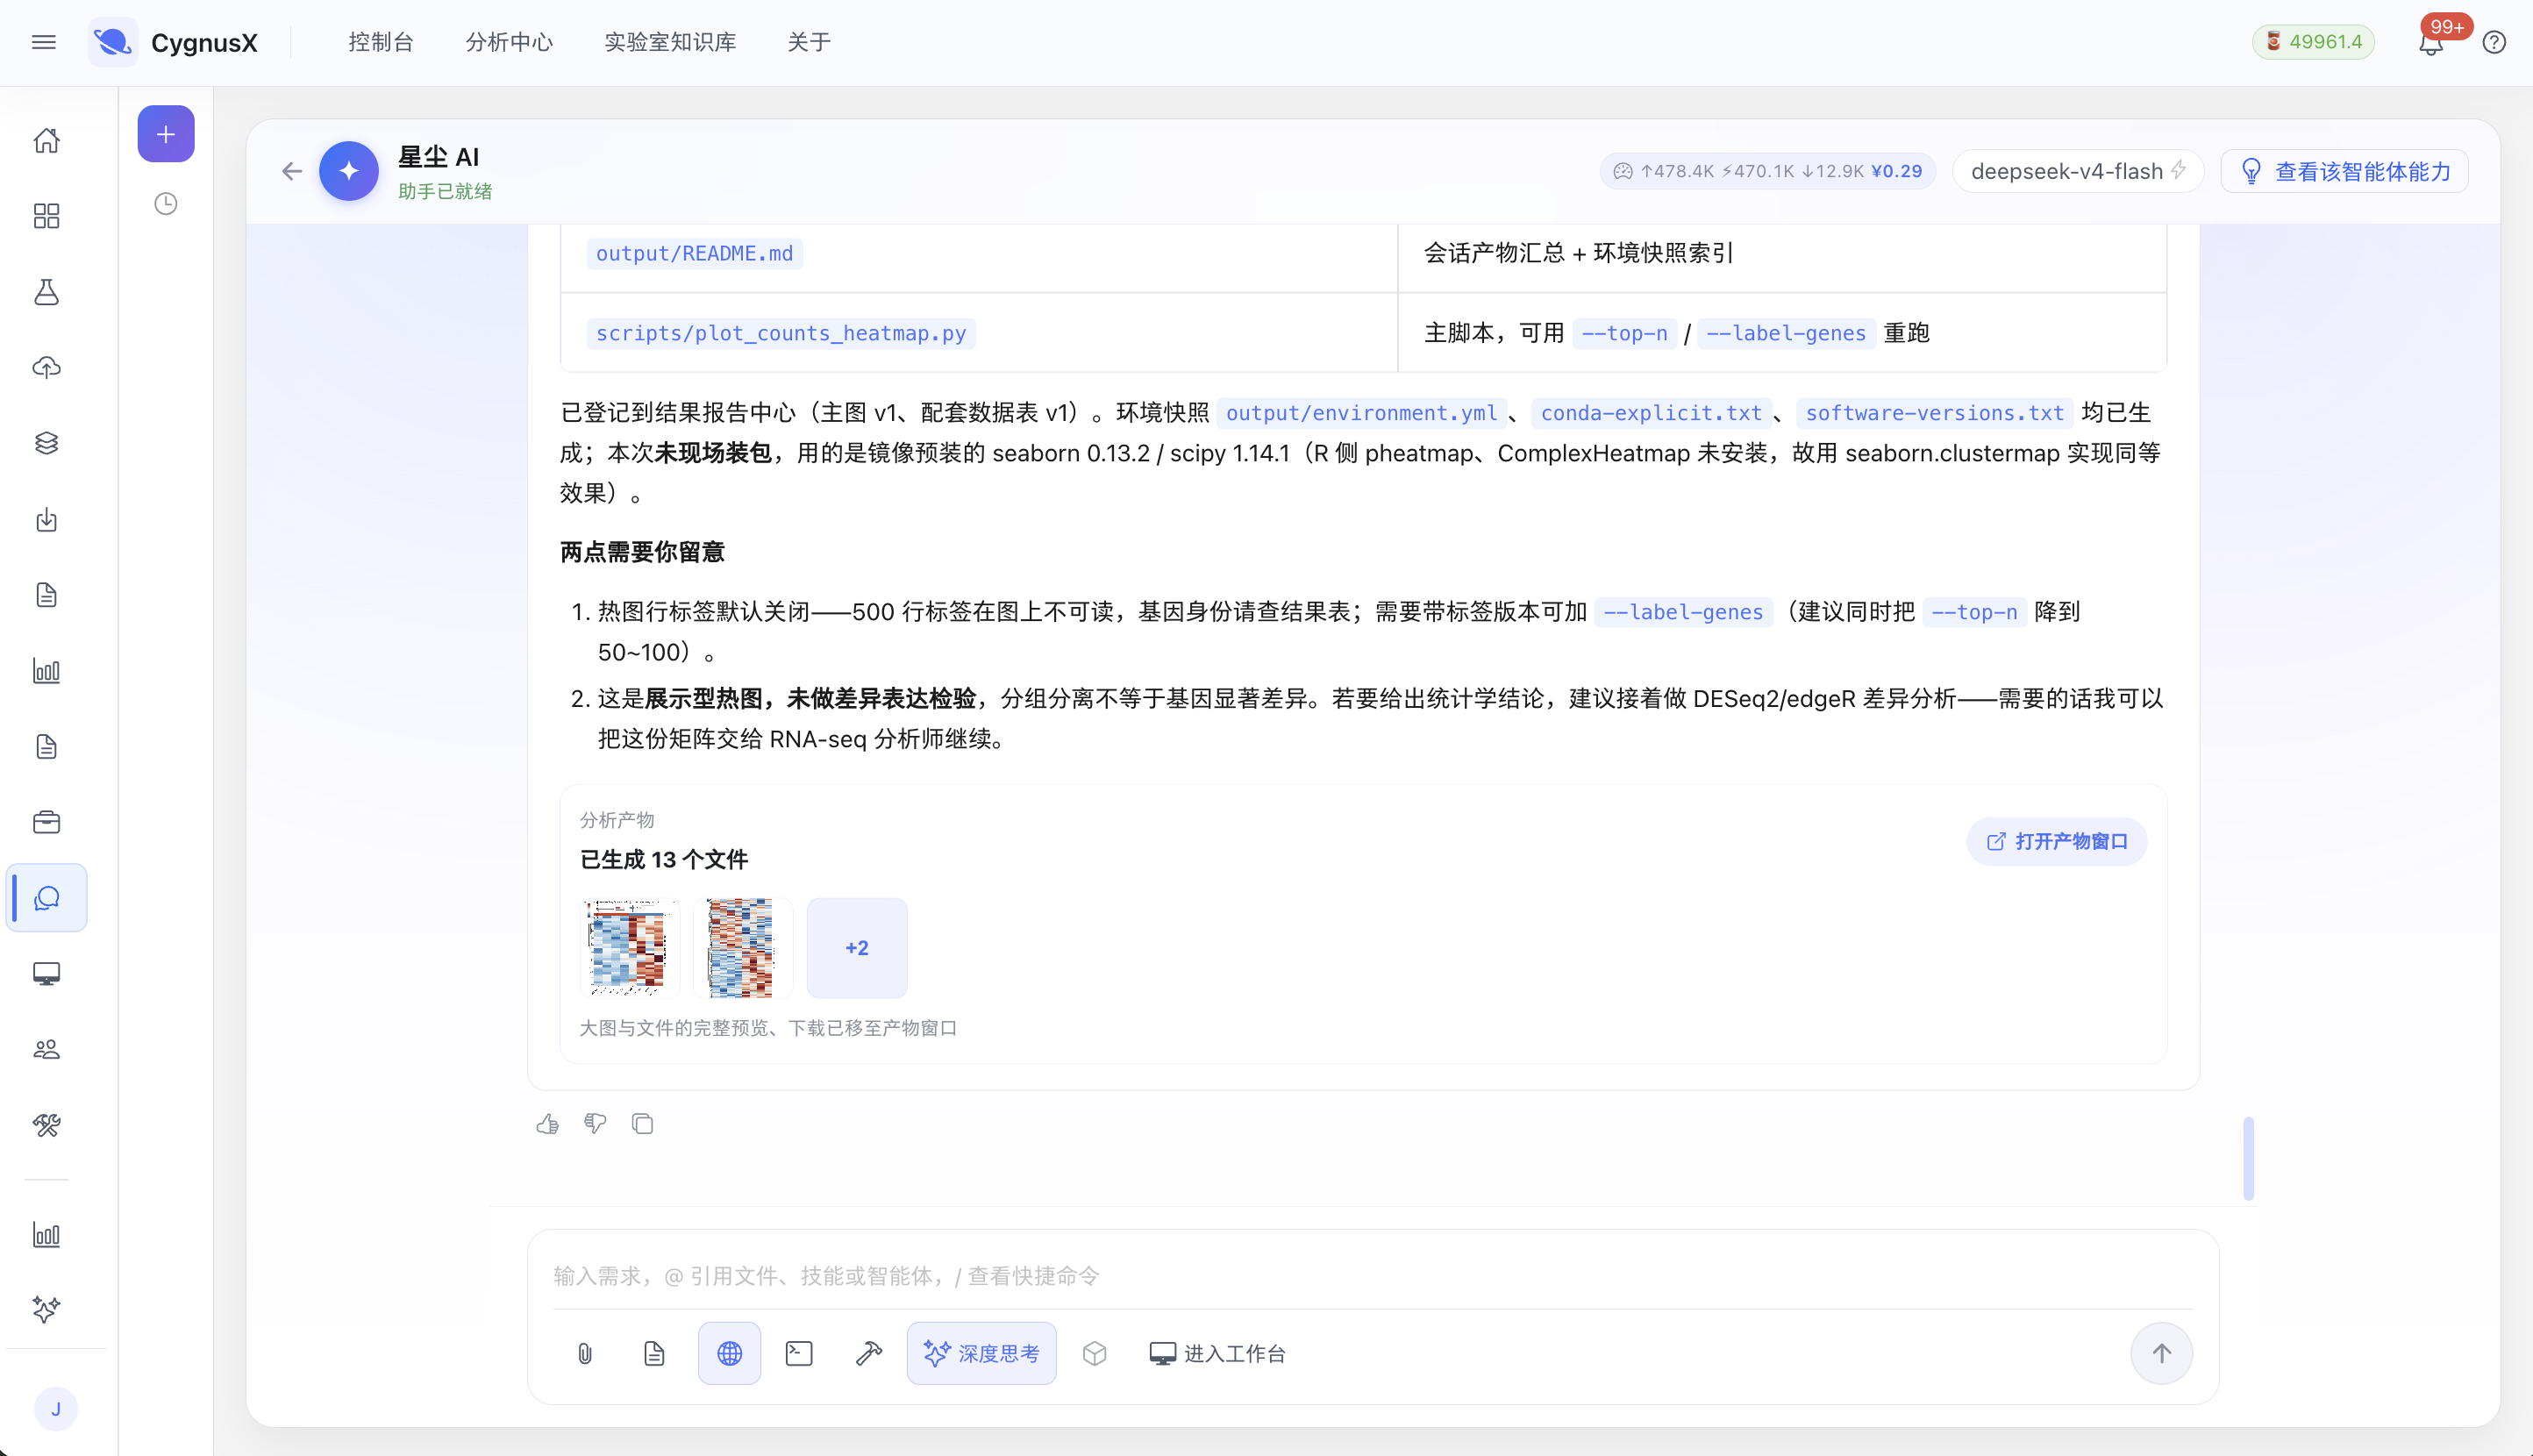
\includegraphics[width=0.95\textwidth]{fig2_evidence_capsule.png}
\caption{Provenance capsule registered automatically by the AI assistant after a task completes. Besides the main result figure and companion data tables, the run also generates \texttt{environment.yml}, \texttt{conda-explicit.txt}, \texttt{software-versions.txt}, and the main script, archived by project ID in the results center for third-party, file-by-file verification.}
\end{figure}

\section{System Implementation and Experimental Quality Control}

\subsection{Layered architecture and local private computing base}

\begin{itemize}
  \item \textbf{Service layer and microservice hub}: an asynchronous high-concurrency framework (FastAPI) covering 29 research microservices and 227 decoupled scientific components, ensuring high responsiveness and isolation when scheduling very large sample cohorts;
  \item \textbf{Scientific data base}: for the I/O pain points of large-capacity omics data (BAM/CRAM/BigWig), \textbf{``in-situ computing''} over local shared storage is implemented, eliminating round-trips to the cloud and meeting the biosafety and compliance requirements of universities and research institutes for highly sensitive genetic resources.
\end{itemize}

\begin{figure}[htbp]
\centering
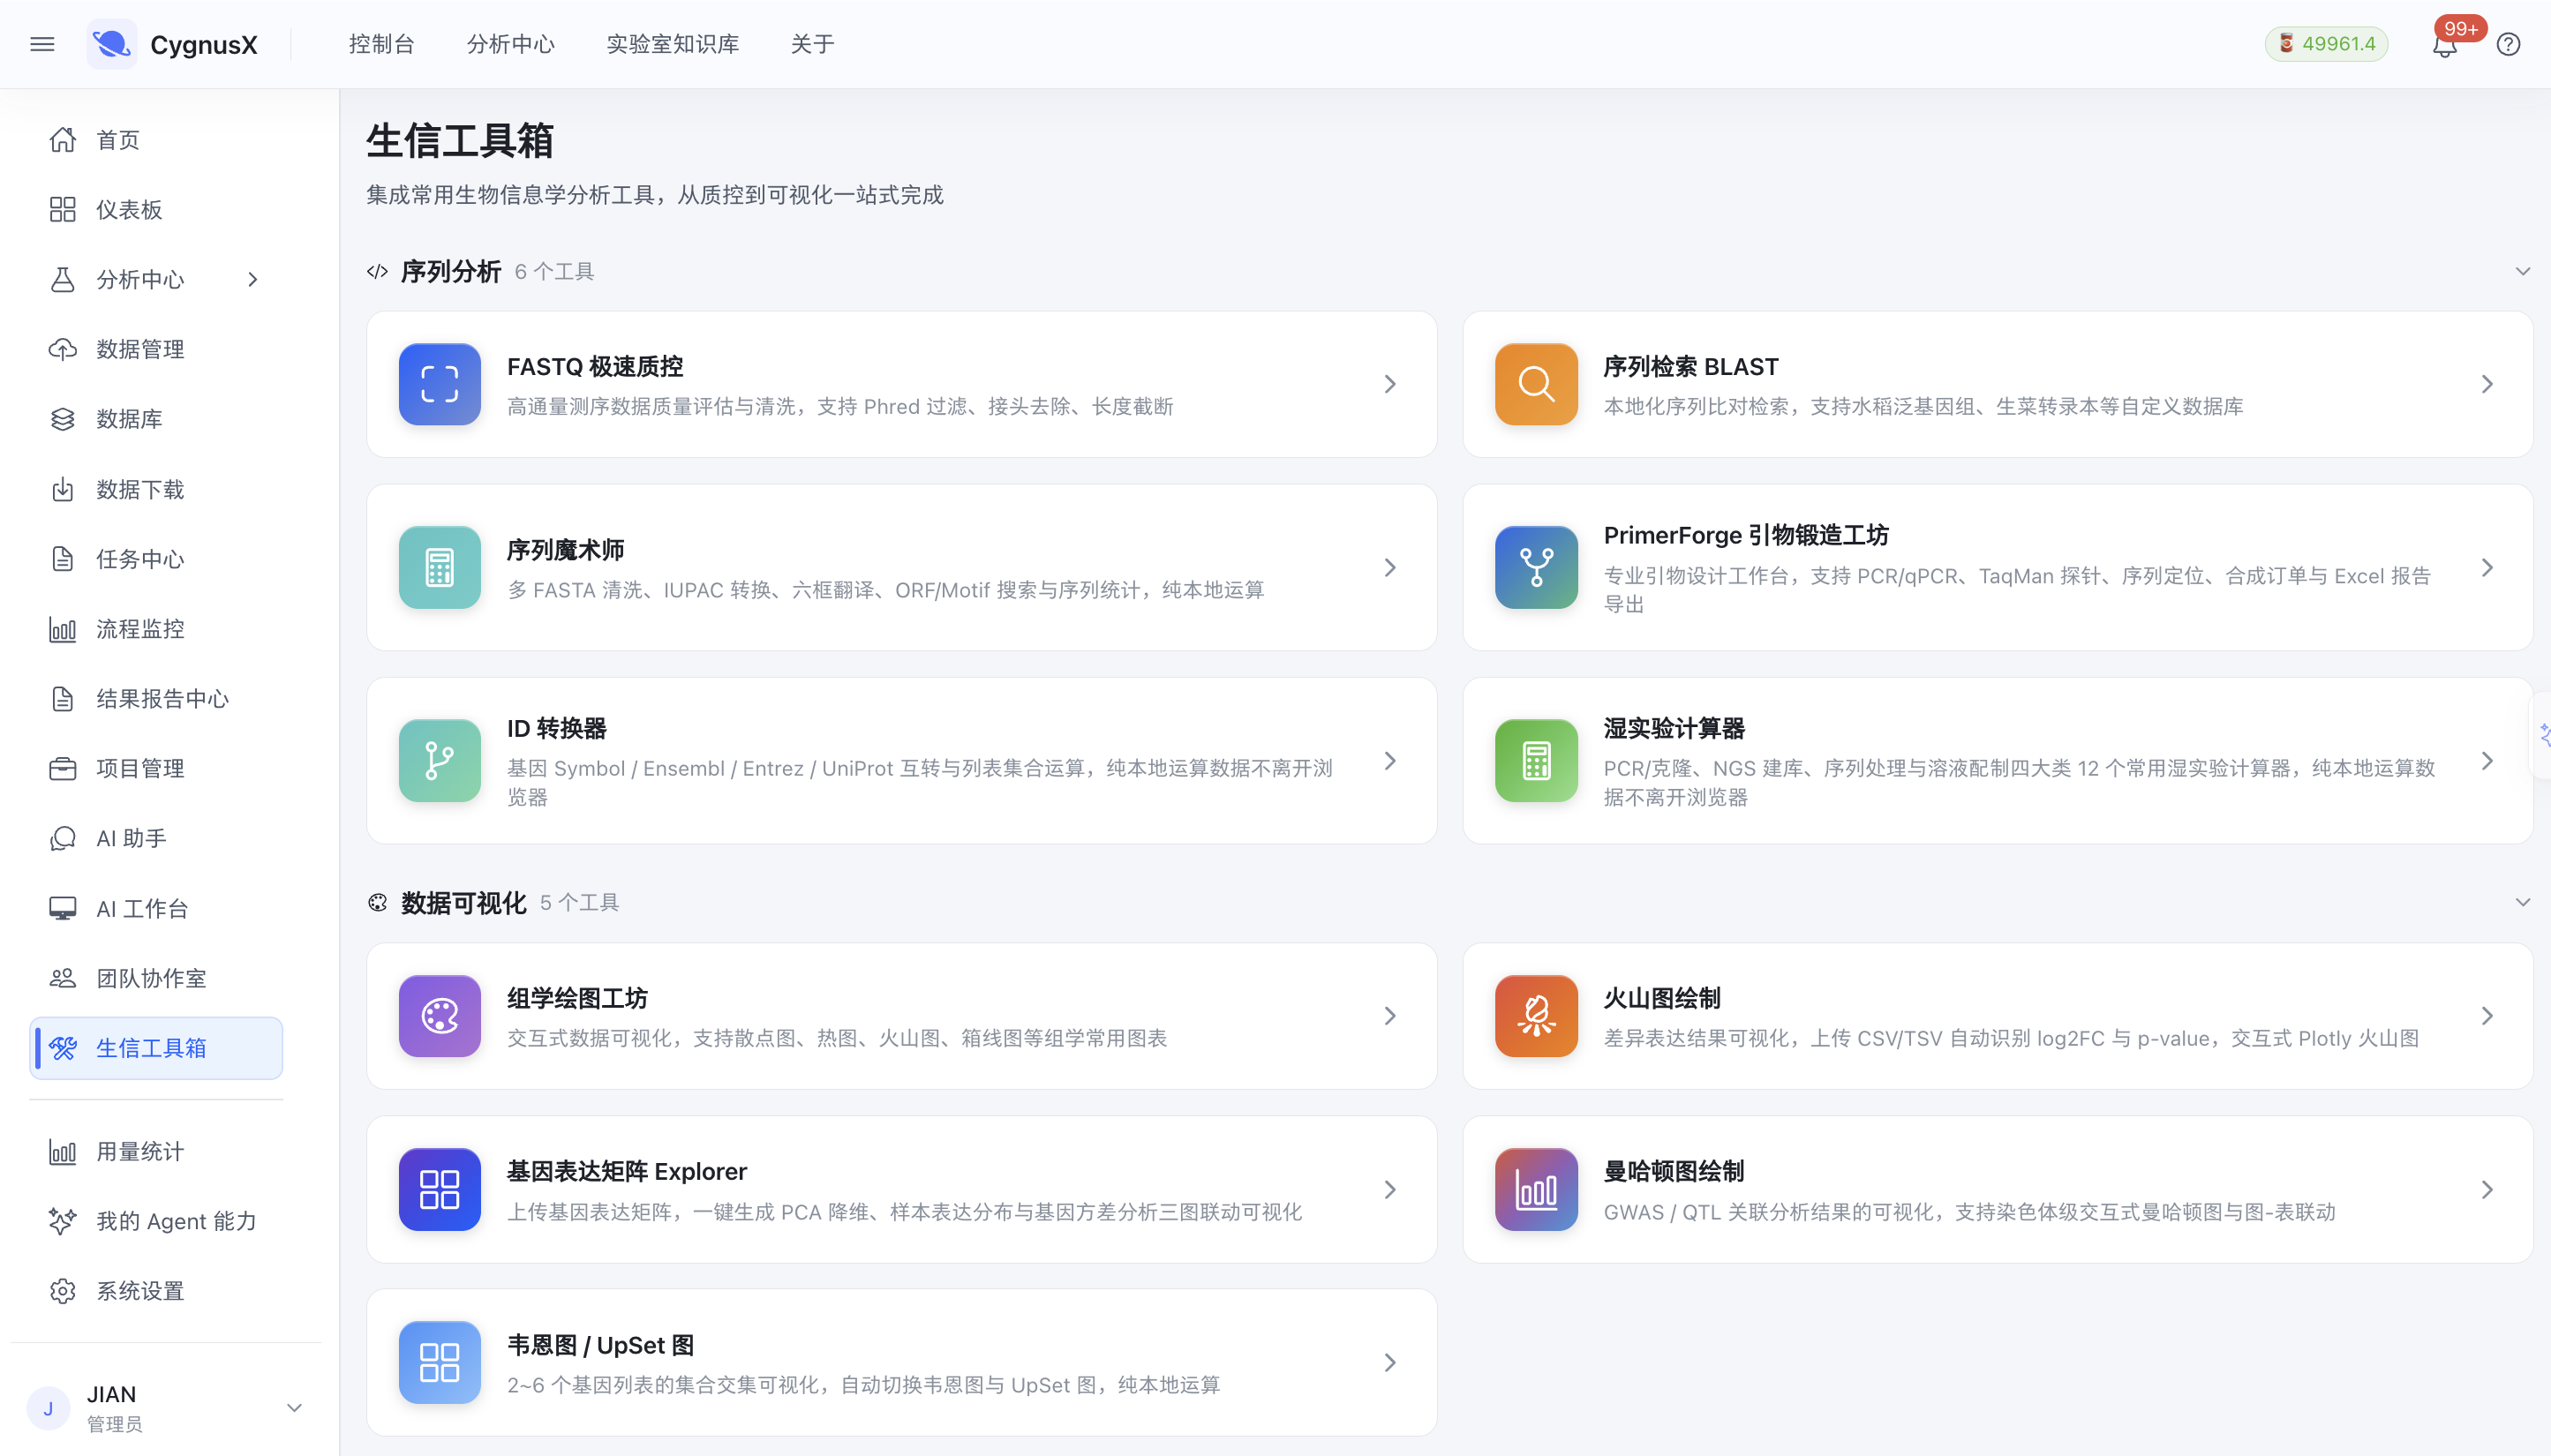
\includegraphics[width=0.95\textwidth]{fig3_bioinfo_toolbox.png}
\caption{Bioinformatics toolbox: a local, unified entry point for conventional tools. Sequence analysis and visualization tools are delivered as web pages; computation runs locally on the server and raw data does not leave the browser environment. This entry shares the same project system and storage interface as the AI assistant and the AI workbench, so the three entries reference shared data logically without repeated copying between tools.}
\end{figure}

\subsection{Rigorous scientific quality gates}

The platform defines three tiers of scientific quality gates:

\begin{verbatim}
[tier 1: static preflight on samples and design]
|- check paired-end matching and the naming contract
|- verify biological replication of control vs treatment groups (>= 3)
\- verify absolute version matching between annotation files (GTF/GFF)
   and alignment indexes

[tier 2: runtime dynamic metric adjudication]
|- sequencing quality control: Q30 ratio, GC-content drift detection
|- alignment effectiveness: unique mapping rate threshold check
\- signal specificity: ATAC-seq TSS enrichment score,
   FRiP (fraction of reads in peaks)

[tier 3: statistical distribution and biological false-positive review]
|- outlier sample detection: unsupervised outlier identification based
   on Cook's distance and hierarchical clustering
\- multiple-testing correction: mandatory FDR / Benjamini-Hochberg
   adjustment to prevent nominal P values from misleading
\end{verbatim}

\section{Core Innovations}

\subsection{Innovation 1: the first ``cognitive reasoning and deterministic computation decoupled'' research multi-agent architecture}

Unlike the unreliable in-industry pattern of relying directly on large models to write bioinformatics scripts, this work confines the long-range logical reasoning and hypothesis-deconstruction ability of the large model to ``top-level planning'' while anchoring data-analysis execution in a rigorous computational framework peer-reviewed by the academic community. The pattern preserves the high interaction flexibility of natural language while delivering the mathematical rigor and determinism that life-science research demands.

\subsection{Innovation 2: a self-closed-loop research decision paradigm centered on the ``causal evidence chain''}

The system breaks through the limitation of conventional pipelines that output only an isolated ``differential gene list''. A professional agent network links the multi-omics dimensions and constructs a cross-omics causal evidence network covering ``epigenetic modification change, chromatin conformational opening, transcriptional activation, and biological pathway cascading''. The system automatically generates scientific explanations with confidence estimates, substantially accelerating the cognitive transformation from data to biological mechanism.

\subsection{Innovation 3: solving the irreproducibility problem of high-throughput computational experiments (Provenance Capsule)}

The platform natively integrates the modern reproducible-science standard into the multi-agent interaction architecture for the first time. Through automatically bound environment-image digests, static algorithm-parameter snapshots, whole-flow MD5 verification, and W3C PROV lineage tracing, every computational experiment attains the high research quality of being ``verifiable ten years later and reproducible across machines and sites''.

\subsection{Innovation 4: the independent check-and-balance mechanism of governance agents improves research rigor}

The ``academic peer reviewer'' mechanism is embedded in the multi-agent system for the first time: the quality-audit agent holds an independent right to block and veto the experiment, and actively intervenes in and self-corrects data-quality defects, potential batch confounding, and inappropriate statistical tests, eliminating ``garbage in, garbage out'' in life-science computational research at its source.

\section{Comparison with the Academic and Industrial Frontier}

In the frontier area where AI for Science meets bioinformatics, representative research results and tool ecosystems exist domestically and abroad. CygnusX differs from them clearly in design paradigm and positioning:

\begin{table}[htbp]
\centering
\renewcommand{\arraystretch}{1.25}
\footnotesize
\begin{tabularx}{\textwidth}{p{0.13\textwidth}X X X X}
\toprule
\textbf{Dimension} & \textbf{Workflow orchestration (nf-core / Galaxy)} & \textbf{Academic frontier agents (BioGPT / GeneGPT / Virtual Lab)} & \textbf{Commercial outsourcing / testing platforms (Novogene Falcon etc.)} & \textbf{CygnusX (this work)}\\
\midrule
Scientific interaction & High-barrier command line / static fixed web forms & Conversational QA / broad literature review & Closed industrial outsourcing delivery interface & \textbf{Hypothesis-driven bidirectional scientific reasoning dialogue + interactive evidence chain}\\
Experiment orchestration & Static DAG pipelines, hard to respond dynamically to hypotheses & Relies on LLM dynamic code generation, error-prone & Pre-fixed commercial pipelines, research logic not customizable & \textbf{Adaptive planning and refactoring of the expert-validated Skill topology}\\
Computational accuracy & High (mature, rigorous tools) & Low (severe code hallucination, obvious statistical defects) & High (standard commercial pipelines) & \textbf{High (cognitive--computational decoupling, rigorously validated statistical kernel)}\\
Reproducibility guarantee & Strong (containers and Conda environments) & Very weak (generated code and randomness differ each run) & Weak (internal enterprise environment, not reproducible externally) & \textbf{Very strong (native W3C PROV provenance capsule + image fingerprint)}\\
Scientific quality governance & Passive post-run static error reporting & Lacks autonomous quality governance and confounder-handling mechanisms & Relies on enterprise QC staff, high cost & \textbf{Built-in quality-audit agent with runtime self-correction and circuit breaking}\\
\bottomrule
\end{tabularx}
\caption{Comparison with representative workflow platforms, academic frontier agents, and commercial platforms.}
\end{table}

\textbf{Core methodological barrier:} academic frontier tools (such as GeneGPT) mainly address knowledge retrieval and small-scale function invocation and cannot handle the heavy computation of GB-scale high-throughput omics long chains; whereas orchestration systems such as Nextflow offer industrial-grade throughput but severely lack intelligent hypothesis deconstruction and scientific explanation. CygnusX sits at the golden intersection of the two: \textbf{endowing industrial-grade rigorous pipelines with scientific intelligence, and endowing large language models with rigorous computational substance.}

\section{Empirical Study and Performance Evaluation}

To fully validate CygnusX's effectiveness on complex life-science problems, the team uses \textbf{``causal regulatory mechanism mining for horticultural crop stress/disease resistance''} as a real research benchmark case.

\subsection{Empirical case: mining multi-omics regulatory targets in the fungal pathogen response}

\textbf{Scientific background and hypothesis input.} A researcher submits the following natural-language scientific question to the platform: ``\emph{24 hours after a plant is infected by a fungal pathogen, identify the core candidate targets of disease defense that are driven by the WRKY transcription-factor family and accompanied by increased chromatin openness.}''

\textbf{Multi-agent autonomous reasoning and collaborative closed loop:}

\begin{enumerate}
  \item The \textbf{experiment-planning agent} rapidly decomposes the complex question into a three-layer computational graph for a dual-omics joint experiment: RNA-seq differential expression modeling + ATAC-seq promoter cis-element analysis + joint enrichment cross-validation;
  \item The \textbf{data-curator and preflight agent} automatically verifies the input dataset (3 replicates Control vs.\ 3 replicates Inoculated), confirms the absence of batch misplacement, and automatically retrieves the corresponding reference-genome annotation;
  \item \textbf{Computational scheduling} activates atomic Skills in sequence (fastp filtering $\rightarrow$ HISAT2 spliced alignment $\rightarrow$ DESeq2 negative-binomial GLM $\rightarrow$ MACS3 peak calling $\rightarrow$ ChIPseeker annotation);
  \item The \textbf{quality-audit agent} monitors in real time, confirming that mapping rate is $> 88.5\%$ and Q30 is $> 93.2\%$ in both sample groups and that signal enrichment at the TSS is significant (score $= 9.8$), and adjudicates the quality gate as passed;
  \item The \textbf{multi-omics integration agent} constructs an evidence causal graph: across layers it localizes 12 core disease-resistance candidate genes (including key PR proteins and receptor kinases) that carry a WRKY-box (W-box: TTGACC/T) in the promoter region, show increased chromatin accessibility (fold change $> 2.1$, $P < 0.001$), and are significantly upregulated at the transcriptional level;
  \item The \textbf{evidence reporter} aggregates a complete research argumentation report combining high-resolution interactive chromatin track plots, differential heatmaps, and GO/KEGG cascade causal interpretation.
\end{enumerate}

\begin{figure}[htbp]
\centering
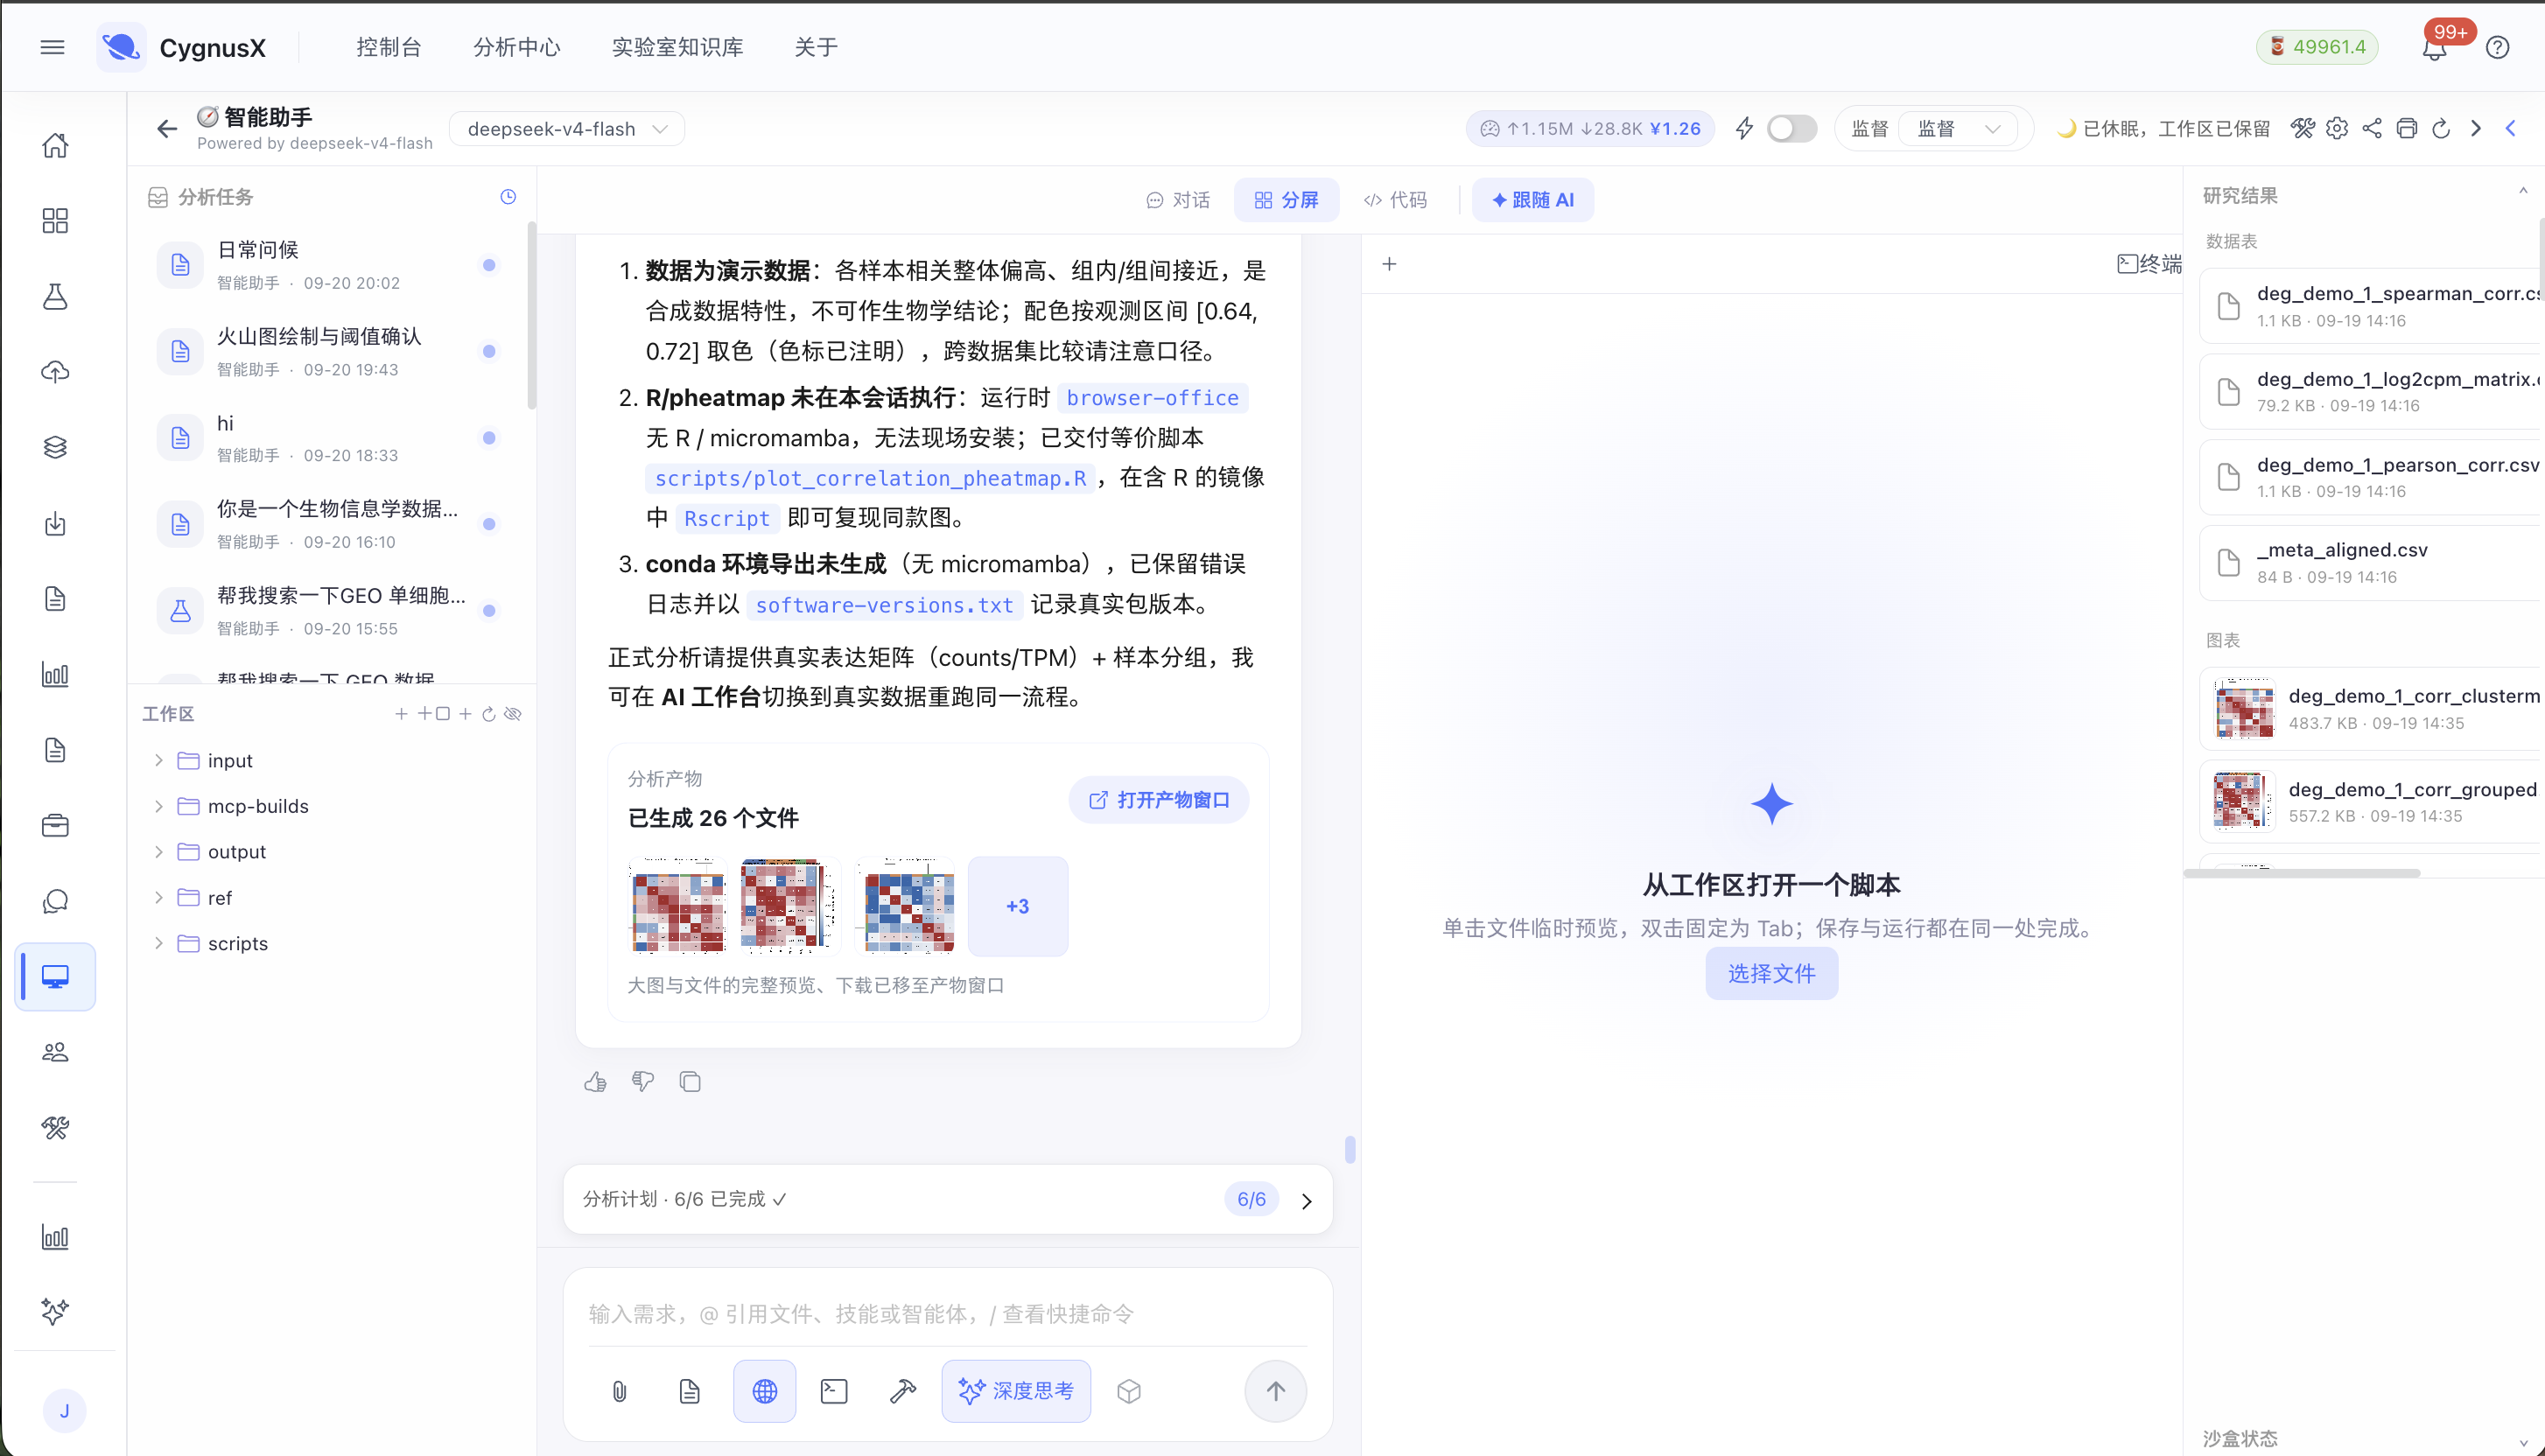
\includegraphics[width=0.95\textwidth]{fig4_ai_workbench.png}
\caption{A differential-expression analysis session in the AI workbench. The left pane is the project workspace (\texttt{input / output / ref / scripts}), the middle pane the session and analysis artifacts, and the right pane the research result tables. Artifacts are registered at file granularity so that scripts and intermediate results are inspectable side by side, ensuring every computation step is traceable.}
\end{figure}

\begin{verbatim}
[scientific hypothesis]
"core defense targets mediated by WRKY after pathogen infection
 with coordinated increase in chromatin openness"
  |
  v
[agent-network collaborative decomposition]
|- RNA-seq path: filtering -> alignment -> negative-binomial
|   differential modeling (DESeq2)
|- ATAC-seq path: peak calling (MACS3) -> promoter cis-open-region
|   identification
\- cross-integration: W-box motif scan -> expression/accessibility
    double-positive causal co-localization
  |
  v
[dynamic quality audit]
OK mapping rate 89.2% | OK TSS enrichment score 9.8 (all gates green)
  |
  v
[causal candidate gene convergence]
35,000+ genes genome-wide -> 840 differentially expressed
  -> 86 with coordinated promoter accessibility
  -> 12 W-box core target genes locked
  |
  v
[full-lifecycle provenance capsule output]
Docker image digest + W3C PROV causal graph + MD5 verification table
+ reproduce_experiment.sh
\end{verbatim}

\subsection{Quantitative research efficiency and computational benchmark}

Under the same test environment, conventional manual analysis by a bioinformatician is compared with the CygnusX platform on complex long-chain tasks:

\begin{table}[htbp]
\centering
\renewcommand{\arraystretch}{1.25}
\begin{tabularx}{\textwidth}{p{0.24\textwidth}X X X}
\toprule
\textbf{Research task metric} & \textbf{Conventional manual analysis} & \textbf{CygnusX platform} & \textbf{Scientific gain}\\
\midrule
Standard dual-omics experiment design and configuration time & $\sim$45 min & $\sim$3 min & \textbf{93\% less time}, substantially reducing low-level engineering friction\\
Incremental hypothesis adjustment (threshold / contrast switch) & $\sim$360 min & $\sim$15 min & \textbf{24$\times$ faster response}, greatly widening hypothesis exploration\\
Cross-omics algorithm reconstruction cycle & $\sim$5 person-days & $\sim$0.5 day & \textbf{90\% shorter engineering cycle}, direct reuse of modular assets\\
Early detection of hidden quality-control errors & Manual experience, often delayed & 100\% automatic static/dynamic interception & \textbf{Eliminates statistical false positives from poor libraries}\\
Third-party laboratory reproduction success rate & Commonly $< 60\%$ (environment drift) & \textbf{100\% (full provenance capsule)} & \textbf{Resolves the computational-experiment reproducibility crisis at its root}\\
\bottomrule
\end{tabularx}
\caption{Reference estimates. Timing includes researcher interaction, inspection, and orchestration waiting time and excludes pure CPU-intensive compute time; calibration against pilot-measured records is required before submission.}
\end{table}

\section{Scientific Value and Roadmap}

\subsection{Research and translation value}

\begin{enumerate}
  \item \textbf{Accelerating plant and animal genomics and breeding}: in crop or horticultural hybridization breeding and stress-trait resolution, the platform helps rapidly filter tens of thousands of variant sites and expression fluctuations, and anchors major regulatory elements with high precision through the multi-omics causal network, substantially shortening the cycle from candidate-gene mining to wet-lab validation.
  \item \textbf{Empowering large core computing platforms in universities and research institutes}: it effectively addresses the pain points of shared bioinformatics facilities --- scarce computational engineers and queues of routine questions and primary analysis requests --- upgrading routine computation into standardized, self-service scientific exploration.
  \item \textbf{Sedimenting the digital intellectual assets of research laboratories}: through standard Skills and canonical workflows, the analysis logic and quality-control conventions of senior bioinformaticians are solidified into transferable code assets, avoiding laboratory technology discontinuity caused by student graduation or staff turnover.
\end{enumerate}

\begin{figure}[htbp]
\centering
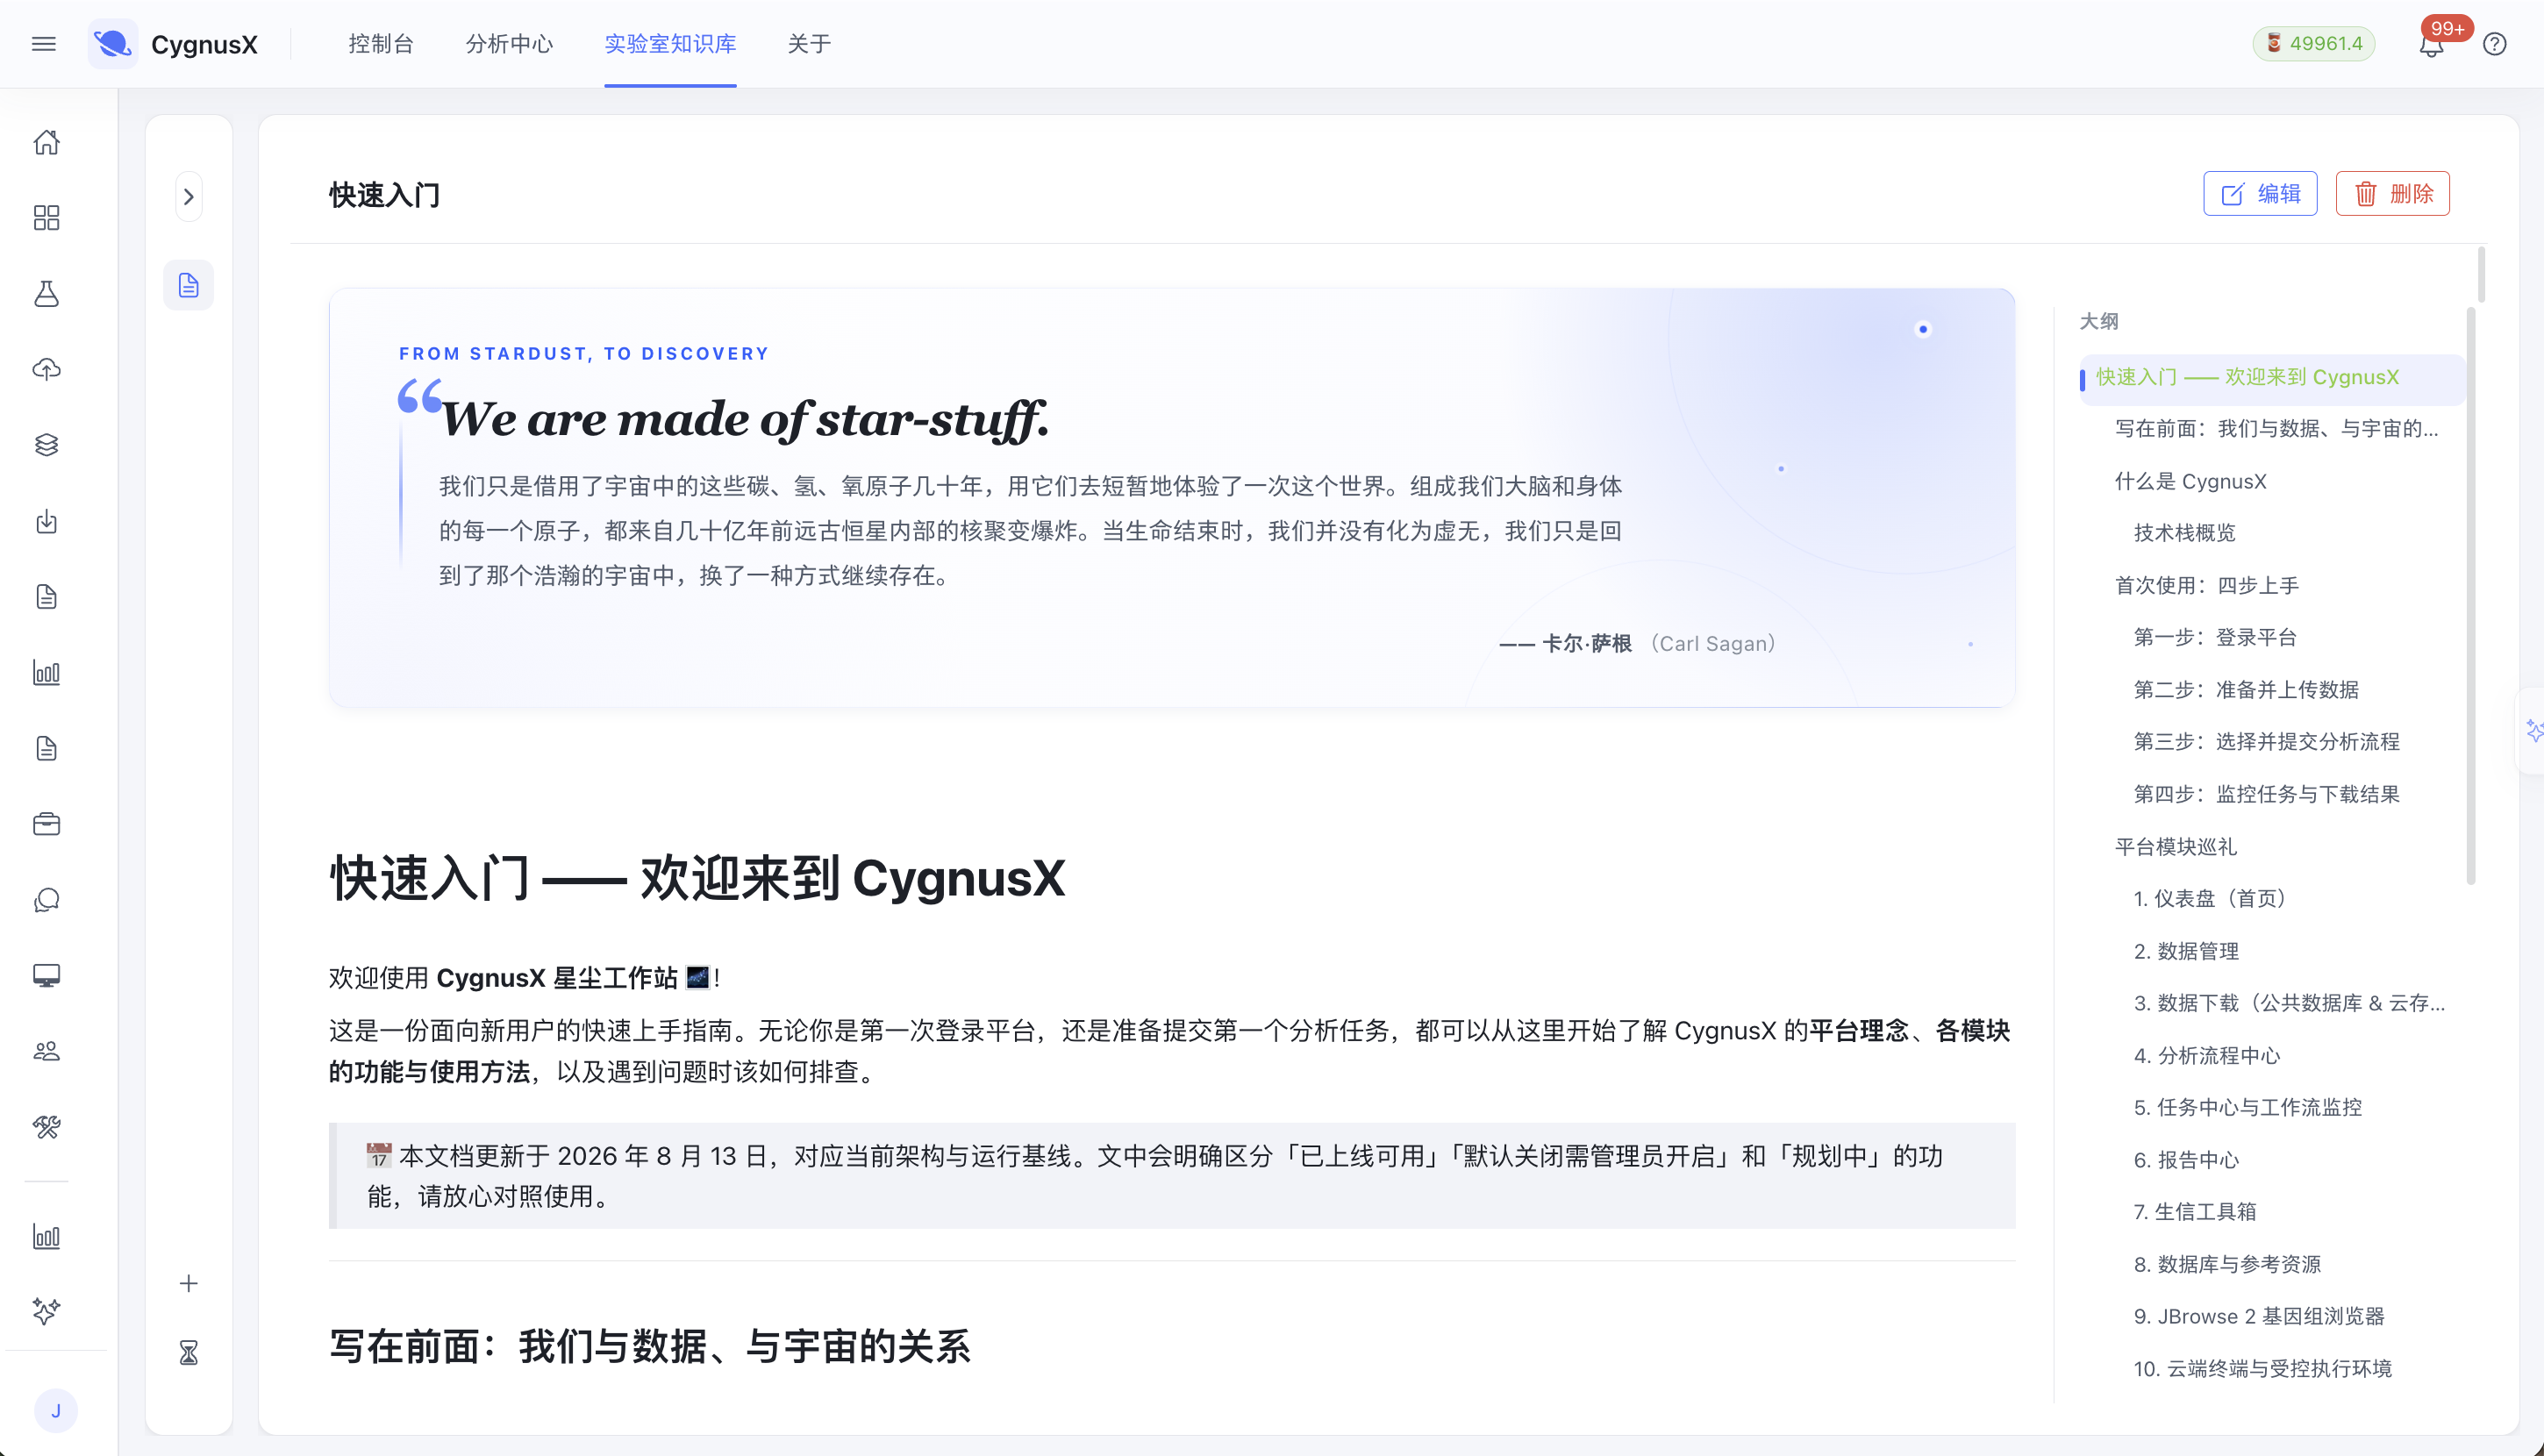
\includegraphics[width=0.95\textwidth]{fig5_knowledge_base.png}
\caption{Laboratory knowledge base: sedimentation and inheritance of research digital assets. Platform philosophy, module tours, operation manuals, and methodology notes are sedimented as structured documentation, with functional status explicitly separated into ``available'', ``disabled by default, admin-enabled'', and ``planned''. Researchers' analysis experience thus leaves personal memory and becomes an inheritable digital asset of the group.}
\end{figure}

\subsection{Roadmap}

\begin{verbatim}
[stage 1: deeper multi-omics coverage (2026 Q4)]
extend scRNA-seq, spatial transcriptomics, and metagenomics domain
agents; build a capability ecosystem of 60+ scientific Skills
  |
  v
[stage 2: linking computational hypotheses with the literature
 knowledge base (2027 H1)]
introduce a domain knowledge graph so that when an agent outputs a
candidate gene set it automatically links the latest PubMed/NCBI
literature for double validation
  |
  v
[stage 3: closed-loop wet-dry robotic exploration (2027 H2+)]
integrate high-throughput automated biological experimental robots,
moving toward "computational hypothesis generation -> automated
experimental testing -> real-time data feedback correction"
\end{verbatim}

\section{Research Ethics, Biosafety, and Data Trustworthiness}

\begin{enumerate}
  \item \textbf{Genetic resource and biosafety compliance}: the platform by design supports \textbf{fully offline private operation} and in-domain in-situ computation. Raw genomic data, clinical phenotypes, or protected genetic resources do not flow through public large models before compliance approval, adhering to the PRC Regulations on the Administration of Human Genetic Resources and biological data-security requirements.
  \item \textbf{Defenses against academic misconduct and model fabrication}: the system adheres to the bottom line of research authenticity and \textbf{strictly forbids any hallucinated data not verified by underlying computation} in generated research reports; every cited statistical significance (P/FDR), correlation coefficient, and enrichment term must be strictly bound to the specific line number and value of the underlying computation output file.
  \item \textbf{AI-assistance disclosure transparency}: all experimental plans and figures output by the system carry a canonical methodological (Methods) draft and a transparent ``AI-assistance disclosure'', consistent with the ethics policies of mainstream journals (such as the Nature and Science families) on the compliant and transparent use of generative AI in scientific research.
\end{enumerate}

\section{Outcomes and Representative References}

\subsection{Project outcomes}

\begin{enumerate}
  \item \textbf{Independent software outcome}: CygnusX computational-experiment platform v0.1.0 (with a complete 18-agent multi-agent system and 38 atomic scientific Skills) \texttt{[add software copyright, papers, awards, or other evidence]};
  \item \textbf{Technical standard accumulation}: produced the ``Omics Atomic Skill Definition and I/O Contract Specification for Multi-Agent Scheduling v1.0'';
  \item \textbf{Empirical case set}: completed cross-omics regulatory mining validation on the high-throughput fungal pathogen response of horticultural plants, producing one complete Provenance Capsule sample \texttt{[add the actual deliverable list]}.
\end{enumerate}

\subsection{Core references}

\begin{enumerate}
  \item Baker, M. 1,500 scientists lift the lid on reproducibility. \emph{Nature} 533, 452--454 (2016).
  \item Koster, J. \& Rahmann, S. Snakemake---a scalable bioinformatics workflow engine. \emph{Bioinformatics} 28, 2520--2522 (2012).
  \item Love, M. I., Huber, W. \& Anders, S. Moderated estimation of fold change and dispersion for RNA-seq data with DESeq2. \emph{Genome Biology} 15, 550 (2014).
  \item Boekel, J. et al. Multi-omic data analysis using Galaxy. \emph{Nature Biotechnology} 33, 137--139 (2015).
  \item Jin, Q. et al. GeneGPT: Augmenting Large Language Models with Domain Tools for Improved Access to Biomedical Information. \emph{Bioinformatics} 40, btae145 (2024).
  \item Bran, A. M. et al. Augmenting large language models with chemistry tools. \emph{Nature Machine Intelligence} 6, 525--535 (2024).
\end{enumerate}

\section{Submission Checklist}

\begin{tabularx}{\textwidth}{p{0.08\textwidth}X X}
\toprule
\textbf{Check} & \textbf{Item} & \textbf{Notes}\\
\midrule
$\square$ & Team ID, unit, and member names and advisor information are complete and correct. & \texttt{IBEC26-35}, Huazhong Agricultural University; members still to be filled\\
$\square$ & Data figures in the performance table and the counts of 29 services, 227 modules, 18 agents, and 38 Skills are verified against the code base. & See repository\\
$\square$ & All ``$>$80\% shorter'' and ``100\% automatic interception'' statements are engineering estimates or design goals and are restated as estimates/pilot figures or backed by measured evidence. & Section 9\\
$\square$ & Version release date, software copyright/papers/awards, the technical specification, and a provenance-capsule example have been added. & Section 12\\
$\square$ & The volume, issue, pages, and year of the six references (Baker, Koster, Love, Boekel, Jin, Bran) have been checked. & Section 12.2\\
$\square$ & High-resolution live screenshots, a sample provenance-capsule directory, and a 3-minute academic demo video are attached. & Figures 1--5 in this report\\
\bottomrule
\end{tabularx}

\end{document}
